%
%\documentclass[a4paper,11pt]{article}
%\usepackage[utf8]{inputenc}	%UTF8 file encoding
%\usepackage[lmargin=3cm,rmargin=4cm,tmargin=3.5cm,bmargin=3.5cm]{geometry}
%\usepackage[T1]{fontenc}
%\usepackage{amssymb,amsmath}
%\usepackage{graphicx, amsthm}
%\usepackage{mathrsfs}
%\usepackage{subcaption}
%\usepackage{color}
%\usepackage{lineno}
%
%\title{Reconstruction}
%\author{}
%\date{\today}
%
%\begin{document}
%\maketitle
%\tableofcontents % table of contents
%\pagenumbering{arabic} % change to arabic numbers
%
%\newpage
%
%\vfill
%
%\section{Reconstruction}


While in the past Cherenkov detectors have been very successful in reconstructing various properties of the particles involved
in a neutrino event, liquid scintillation detectors have long been thought as a source for calorimetric information only. 
However, in recent years it became obvious that the time information of the light in liquid scintillators can be used to 
access a wide range of information, similar or even superior to what a pure Cherenkov detector can deliver. 

Basically, there are two complementary approaches to reconstruction in both detector types and consequently also in WBLS 
detectors. The first approach developed in MiniBooNE [] and successfully applied in T2K [] follows a likelihood ansatz to 
find the optimal track parameters and compare different hypotheses. In contrast to this, the three-dimensional topological 
reconstruction tries to picture the spatial distribution of the energy deposition within the detector without using a 
specific hypothesis. This technique has been developed for the LENA [] detector and successfully been used for muon events 
in Borexino. These are liquid scintillator detectors, but the application to Cherenkov detectors is straight forward. 

Both methods have been improved considerably over the last couple of years. For example fitQun, the reconstruction software 
used by T2K is now able to reconstruct up to 6 Cherenkov rings. This alone will increase the expected sensitivity 
for example for CP-violation in the LBNF beam significantly in comparison to previous studies like []. In addition, the 
topological reconstruction promises large volume liquid detectors the same capabilities as only highly segmented detectors 
used to have (with all the implications of that). This includes possibilities for particle identification at energies as low as
a few MeV based on topological information. This ability will be further enhanced by the combination of the two light species,
Cherenkov and scintillation light, as can be seen in [Andrey], where Cherenkov-Scintillation separation is used to
identify the two electrons of a 0$\nu\beta\beta$-decay.

To give an overview on the state of the art in reconstruction, this section is divided into four subsections. The first
subsection is dedicated to the likelihood approach and its latest results. The second subsection describes the topological 
reconstruction and its application to high energy events at the GeV scale and low energy events at the MeV scale. The third 
subsection is dedicated to applications of Cherenkov-light-Separation at low energies. Finally,  we comment 
on other approaches like …..

\subsection{Likelyhood}

This subsection summarizes the main features of the reconstruction 
method developed for the MiniBooNE detector\cite{ryanpaper}. In this 
method a likelihood function is evaluated for a particle (particles) of some type
with initial kintmatic parameters to have produced the observed collection 
of PMT hits, charges and times, in an event. A key ingredient 
of the likelihood calculation is the predicted hit distribution which 
represents the average response of the detector for such a particle and
therefore the likelihood is a function of the paricle's kinematic parameters. 
The optimal parameters would provide the best agreement between
the predicted and observed hit distributions i.e. the likelihood
function will be at a maximum.

Realistic model of detector response is required to develop a
successful and efficient event reconstruction and identification algorithms.
This requires both {\it in-situ} and {\it ex-situ} measurements
of various optical properties of the water, PMTs and the reflection
of all surface inside the detector. Absorption, scattering, reflections
and fluorescence processes can affect the reconstruction.
In order to account for these effects in the reconstruction,
these optical properties have to be obtained if unknown. 

Single track is parametrized with 7 parameters: starting point $(x_0, y_0, z_0)$,
starting time $t_0$, direction $\theta_0, \phi_0$ with respect to the beam
and kinetic energy $E_0$. We refer to this vector as ${\bf u}$.
Track information is obtained by maximizing the likelihood that
track with vector ${\bf u}$ will produce the observed PMT
measurements. The likelihood for an event assuming all PMTs are independent
is given by

\begin{equation}
	L({\bf q, t; u})=\prod_i^{N_{unhit}} P_i(\text{unhit}; {\bf u})\times\prod_j^{N_{hit}} P_j(\text{hit}; {\bf u})f_q(q_j;{\bf u}) f_t(t_j;{\bf u}).
\end{equation}
Here $P_i(\text{unhit}; {\bf u})$ is the probability PMT $i$ is not hit given ${\bf u}$,
$P_i(\text{hit}; {\bf u})$ is the probability PMT $i$ is hit given ${\bf u}$,
$f_q(q_j;{\bf u})$ is the probability density function for the measured charge $q$ given ${\bf u}$ and
predicted charge $q_j$,
$f_t(t_j;{\bf u})$ is the probability density function for the measured time $t$ given ${\bf u}$
evaluated time $t_j$. Product is carried over all PMTs. For convenience 
we can work with the negative logarithm of the likelihood which can 
be written as a sum of negative logarithms. We will use $F_q$ and $F_t$ to denote the
charge and the time negative logarithm likelihoods respectively  
\begin{equation}
	-\log L({\bf u}) \equiv F_q({\bf u}) + F_t({\bf u}),
\end{equation}

\begin{equation}
	F_t({\bf u}) = -\sum_i^{N_{hit}} \log f_t(t_i;{\bf u}),
\end{equation}

\begin{equation}
	F_q({\bf u}) = -\sum_i^{N_{unhit}}\log P_i(\text{unhit}; {\bf u})-\sum_i^{N_{hit}}\log P_i(\text{hit}; {\bf u}) - \sum_i^{N_{hit}} \log f_q(q_i;{\bf u}).
\end{equation}
From here on we will refer to $F_q$ and $F_t$ simply as the charge and the time likelihoods.

If the number of observed photoelectrons (PE), $n_i$, is known for a given PMT one can assume
that $f_q(q_i;{\bf u})$ is fully specified regardless of detector properties.
In addition, $n_i$ can be assumed to be Poisson distributed with a mean value
$\mu_i({\bf u})$ (predicted charge) for which the notation $\mu_i$ will be
used with implicit dependence on ${\bf u}$. As a result, the probability
for a PMT to have no hit is
\begin{equation}
	P_i(\text{unhit}; {\bf u})\equiv\overline P_i(\mu_i)=e^{-\mu_i}.
\end{equation}
Hence, the probability a PMT has recorded a hit is
\begin{equation}
	P_i(\text{hit}; {\bf u})\equiv P_i(\mu_i)=1-\overline P_i(\mu_i).
\end{equation}
The next step is to separate the predicted charge into prompt and late predicted charge
\begin{equation}
	\mu_i \equiv \mu_{prompt,i} + \mu_{late,i}.
\end{equation}
The prompt predicted charge is a result of \v{C}erenkov light, while the
late predicted charge has contributions from direct \v{C}erenkov light and
indirect light. Sources of indirect light are reflections, scattering and 
fluorescence.

Time PDFs $f_t(t_i;{\bf u})$ depend on the first photon to fire
the PMT. Dependence on ${\bf u}$ can be reduced by introducing
corrected time
\begin{equation}
	t_{cor,i}=t_i-t_0-\frac{r_{mid,i}(E_0)}{c_n}-\frac{\Delta s_{mid}(E_0)}{c},
\end{equation}
where $t_i$ is the measured PMT time, $t_0$ is the measured start time,
$\Delta s_{mid}(E_0)$ is the distance from the track start point to
the mean \v{C}erenkov emission point, $r_{mid,i}(E_0)$ is the distance
from the mean \v{C}erenkov emission point to the PMT, $c_n$ and $c$ are
the speeds of light in water and vacuum respectively. 
Due to the latency period PMT can register only one hit for a given track.
Probabilities of no prompt PEs and no late PEs can be written as
$P(\text{no prompt PEs}) = e^{-\mu_{prompt}}$ and $P(\text{no late PEs}) = e^{-\mu_{late}}$ 
respectively. The probability that a hit contains at least one prompt PE is
\begin{equation}
	w_p=P(\text{prompt PE present}|hit) =\frac{1-P(\text{no prompt PEs})}{1-P(\text{no prompt PEs})P(\text{no late PEs})}.
\end{equation}
This is the weight for the prompt primitive distribution $G_{ch}(t_c,E_0,\mu_{prompt})$, while the $w_l=1-w_p$ is the
weight for the late primitive distribution $G_{late}(t_c,E_0,\mu_{late})$. Finally, the time PDF is
obtained from
\begin{equation}
	f_t(t;E_0,\mu_{prompt},\mu_{late})=w_p G_{ch}(t_c,E_0,\mu_{prompt})+w_l G_{late}(t_c,E_0,\mu_{late}).
\end{equation}
The primitives distribution are created by generating particles throughout the detector in
special runs (e.g. only \v{C}erenkov light and no scattering) and the response is parametrized. 

\subsection{3D topological reconstruction}

In this subsection a reconstruction method is presented which aims to provide a 3D topological representation of the energy 
deposition of an event.
%The aim of the reconstruction methods presented in this section is to provide a 3d topological representation of the energy deposition of an event. 
As the topology in question can have an arbitrary form, a method is needed which is not based on a hypothesis concerning the event
type or rather the geometrical appearance of the energy deposition. Therefore, the only assumptions made within this method are 
that a reference point on the topology is known reasonably well in space and time (the time of the energy deposition) and that 
all particles propagate through this point in approximately straight lines with the speed of light. The necessary reference point 
has to be provided by a prior analysis of the event. In order to get information not only on likely points of energy deposition 
but also on the amount of energy deposit at each point, the full timing information of an event has to be used. This is in contrast
to the other two methods in this paper where only the time of the first hit of each PMT is exploited. In the case that only the 
first hit time is known, this method can - after some adaptations - still be useful to provide pure topological information but 
the amount of energy deposition at each point is not easily reconstructable.


%The only requirement is the knowledge about one point in space and time where

%In this section

%motivation 
%binned
% can be adapted for first hits only, but this will not be discussed here


\subsection*{Basic idea}
\label{Sec:BasicWonsakReco}

  The general idea here is to use the timing information of all registered signals for the construction of isochronal surfaces around each 
  light sensor defined by the signal time. The overlap of these surfaces then indicates likely points of origin of the detected photons 
  and thus can reflect the spatial distribution of the energy deposition of an event. For a point-like photon emission source each 
  signal time corresponds to a spherical surface around the light sensor (PMT)\footnote{Since PMTs are still the most common light sensors used in large 
  volume liquid detectors, we will refere to the light sensors as PMTs in the following text. However, in principle every kind of
  light sensor is suited as long as it can detect single photons.}. By overlapping spheres around different PMTs the point 
  source can then be located. For extended events this approach has to be modified, because it is not clear from which point of 
  the event topology a given detected photon originated. Thus the time of flight of the particle acts as an offset to the signal 
  arrival time. Therefore, the ansatz of simply using spheres with a radius corresponding to the time of the signal is limited. 
  However, with some very simple approximations similar surfaces can be generated for extended events.
  %However, spheres can be very effective in extracting vertex positions, when using only the first hit of each PMT.
  
  %---------- FIGURE BEGIN ----------%    
\begin{figure}[b!t]
  \centering
    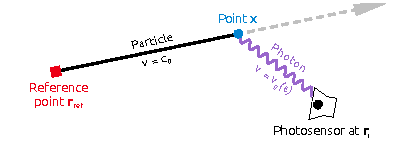
\includegraphics[width=0.70\textwidth]{recon/reco_signal_transport_concept.pdf}
    \caption{Illustration of the basic part of the information transport model used in the 
topological reconstruction. Passing the reference point $\bvec{r}_{\mathrm{ref}}$ at the
reference time $t_{\mathrm{ref}}$, a charged particle travels with the speed of light in vacuum
$c_0$ along a straight track through $\bvec{x}$. A photon thereby emitted with energy $\epsilon$ at 
point $\bvec{x}$ reaches the photosensor at $\bvec{r}_j$ with the speed equal to the 
energy-dependent group velocity $v_g(\epsilon)$.}
  \label{fig:InfoTransportModel}
\end{figure}
%---------- FIGURE END ----------%
  
  We only have to assume that all particles involved in an event propagate with the speed 
  of light $c$ directly away from the primary vertex. The total time $t_{signal}$ between the start of the event and the arrival
  time of a scintillation photon at a given PMT can then be separated into two parts: 
  The time it takes for the particle to propagate from the vertex $V$ to the emission point $X$ of the scintillation photon and the
  time the scintillation light needs from this emission point to reach the PMT~$P$. This leads to the equation

%  Given this knowledge and assuming, that all particles involved in an event propagate with the speed of light directly away from the primary vertex, it is possible 
%  to correct for the propagation time of the particles involved considering the equation

 \begin{equation}
   \label{Eq:Drop-like_shape}
%  c \cdot t_{signal} = \abs{\bar{VX}} + n \abs{\bar{XP}} \; ,
  c \cdot t_{signal} = \abs{|\overline{VX}|} + n \cdot \abs{|\overline{XP}|} \; ,
 \end{equation}
%
  where
  %the signal time $t_{signal}$ is the time between the first interaction at the vertex $V$ and the arrival of an optical photon at a PMT $P$, 
  $n$ is the effective refraction index for the scintillation light, $\abs{|\overline{VX}|}$ is the distance between the vertex $V$ of 
  the event and the point of photon emission $X$, while $\abs{|\overline{XP}|}$ is the distance between the point $X$ and the PMT $P$ (see Fig. \ref{fig:InfoTransportModel}). This 
  formula describes surfaces which have a drop-like shape as seen in Fig. \ref{fig:DropShapes}. This implies that -- given a prior knowledge of 
  the vertex and the time of the interaction at this point -- drop-like surfaces can be constructed around each PMT $P$ which contain 
  all the possible points of origin $X$ for a signal arriving at a time $t_{signal}$. Overlapping these drop-like surfaces of all signals
  involved will then give an impression of all points where photons have been generated, i.e. the event topology. 
  
  Several important aspects have to be noted at this point. First, it is essential to have a reference point on the event topology. The natural
  choice for this reference point is the primary vertex, but any point on the topology is suitable. However, if the reference point is 
  not the primary vertex, a second set of surfaces is necessary instead of only using the drop-like shapes. This second type of surfaces 
  occurs if you allow parts of the topology to lie backward in time with respect to the reference point. Then, Equation \ref{Eq:Drop-like_shape}
  has to be modified with a minus sign in front of the propagation part $\abs{|\overline{VX}|}$ and thus every signal produces a 
  second hyperbola-like surface which also contributes to the set of allowed points of origin for every detected photon. For the sake 
  of simplicity, we will always assume in the following that we know the primary vertex with sufficient accuracy. 
  %This is a justified presumption, as becomes evident from the results of the backtracking algorithm presented in Section \ref{}. 
  
  % ---------- FIGURE BEGIN ----------%
\begin{figure}[b!t]
  \centering
  \begin{subfigure}[t]{0.48\textwidth}     
    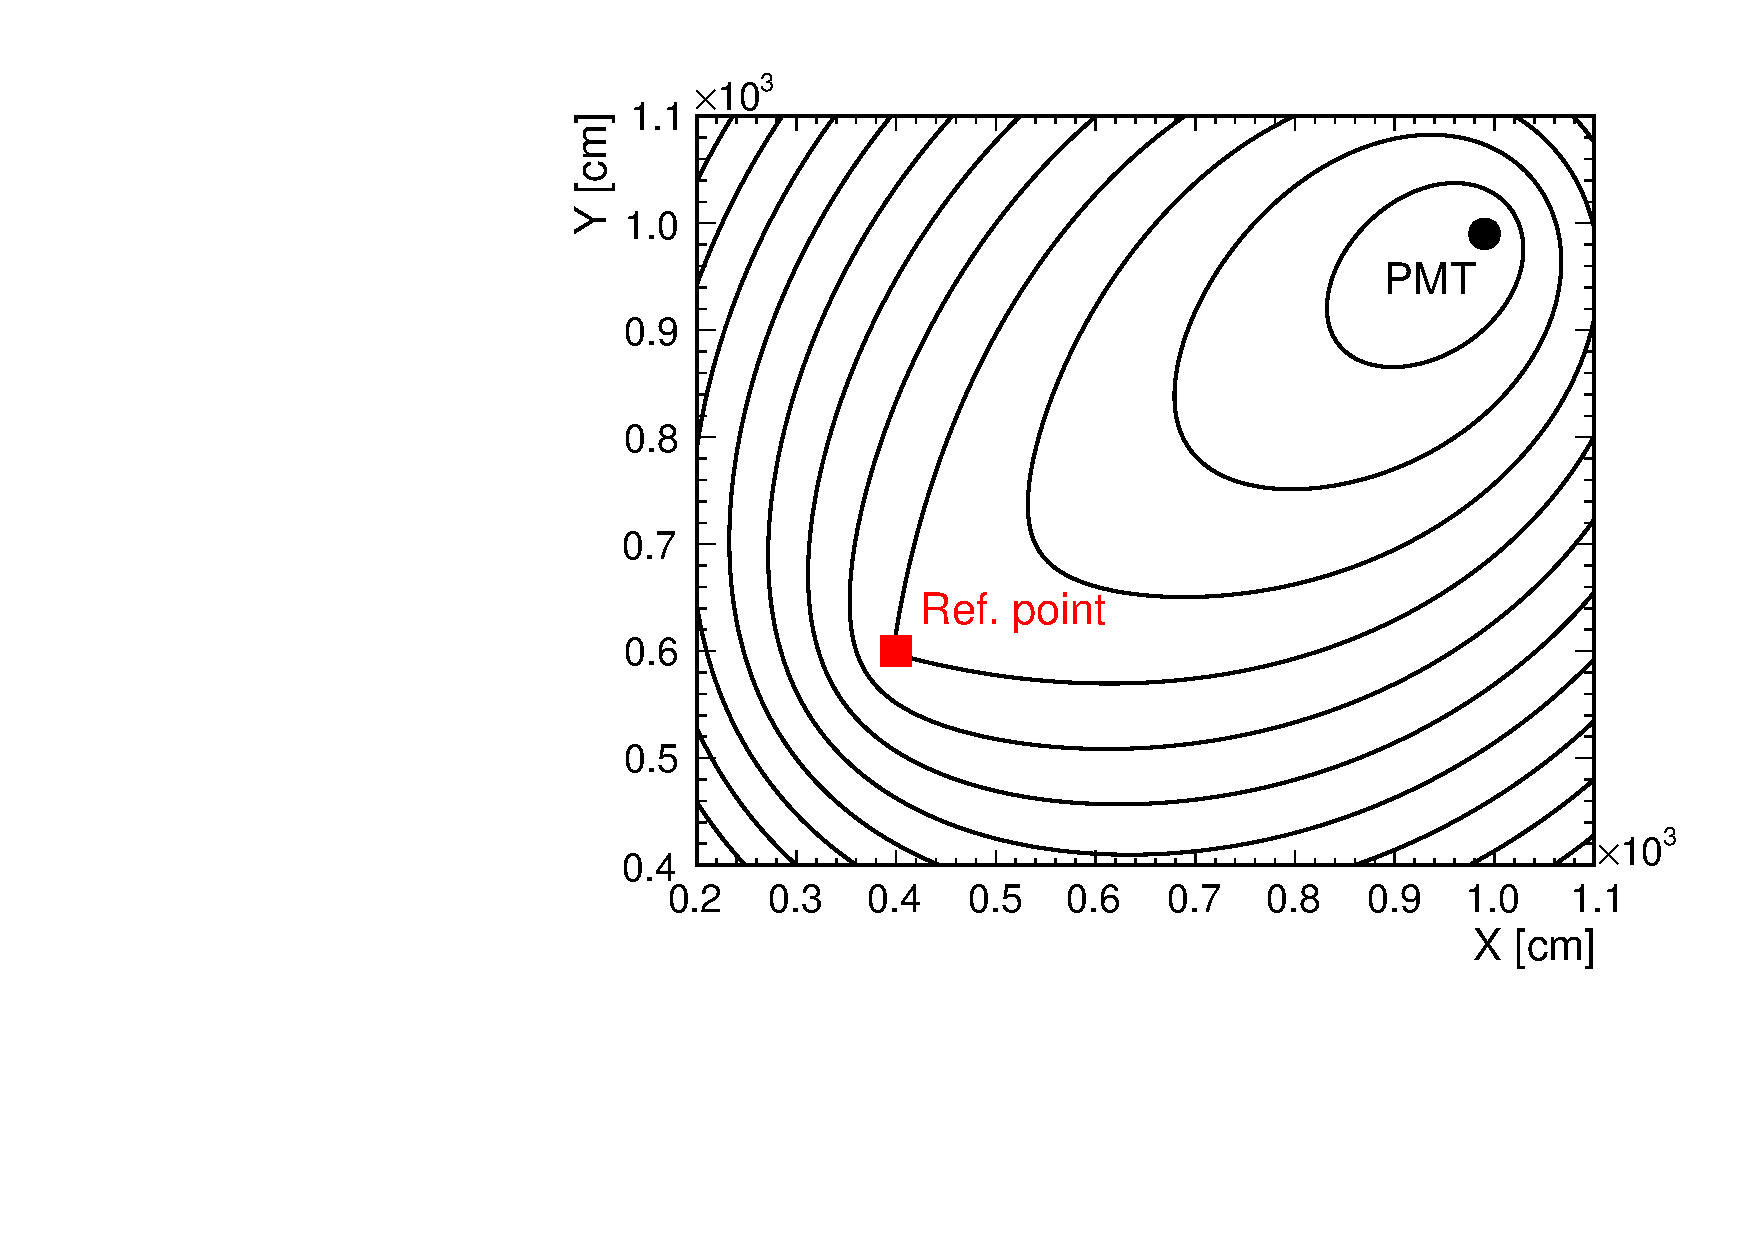
\includegraphics[trim=0.1cm 0.1cm 0.5cm 0.1cm,clip=true,width=\textwidth]
      {recon/DropShape_forward.pdf}
  \end{subfigure}
  ~
  \begin{subfigure}[t]{0.48\textwidth}
    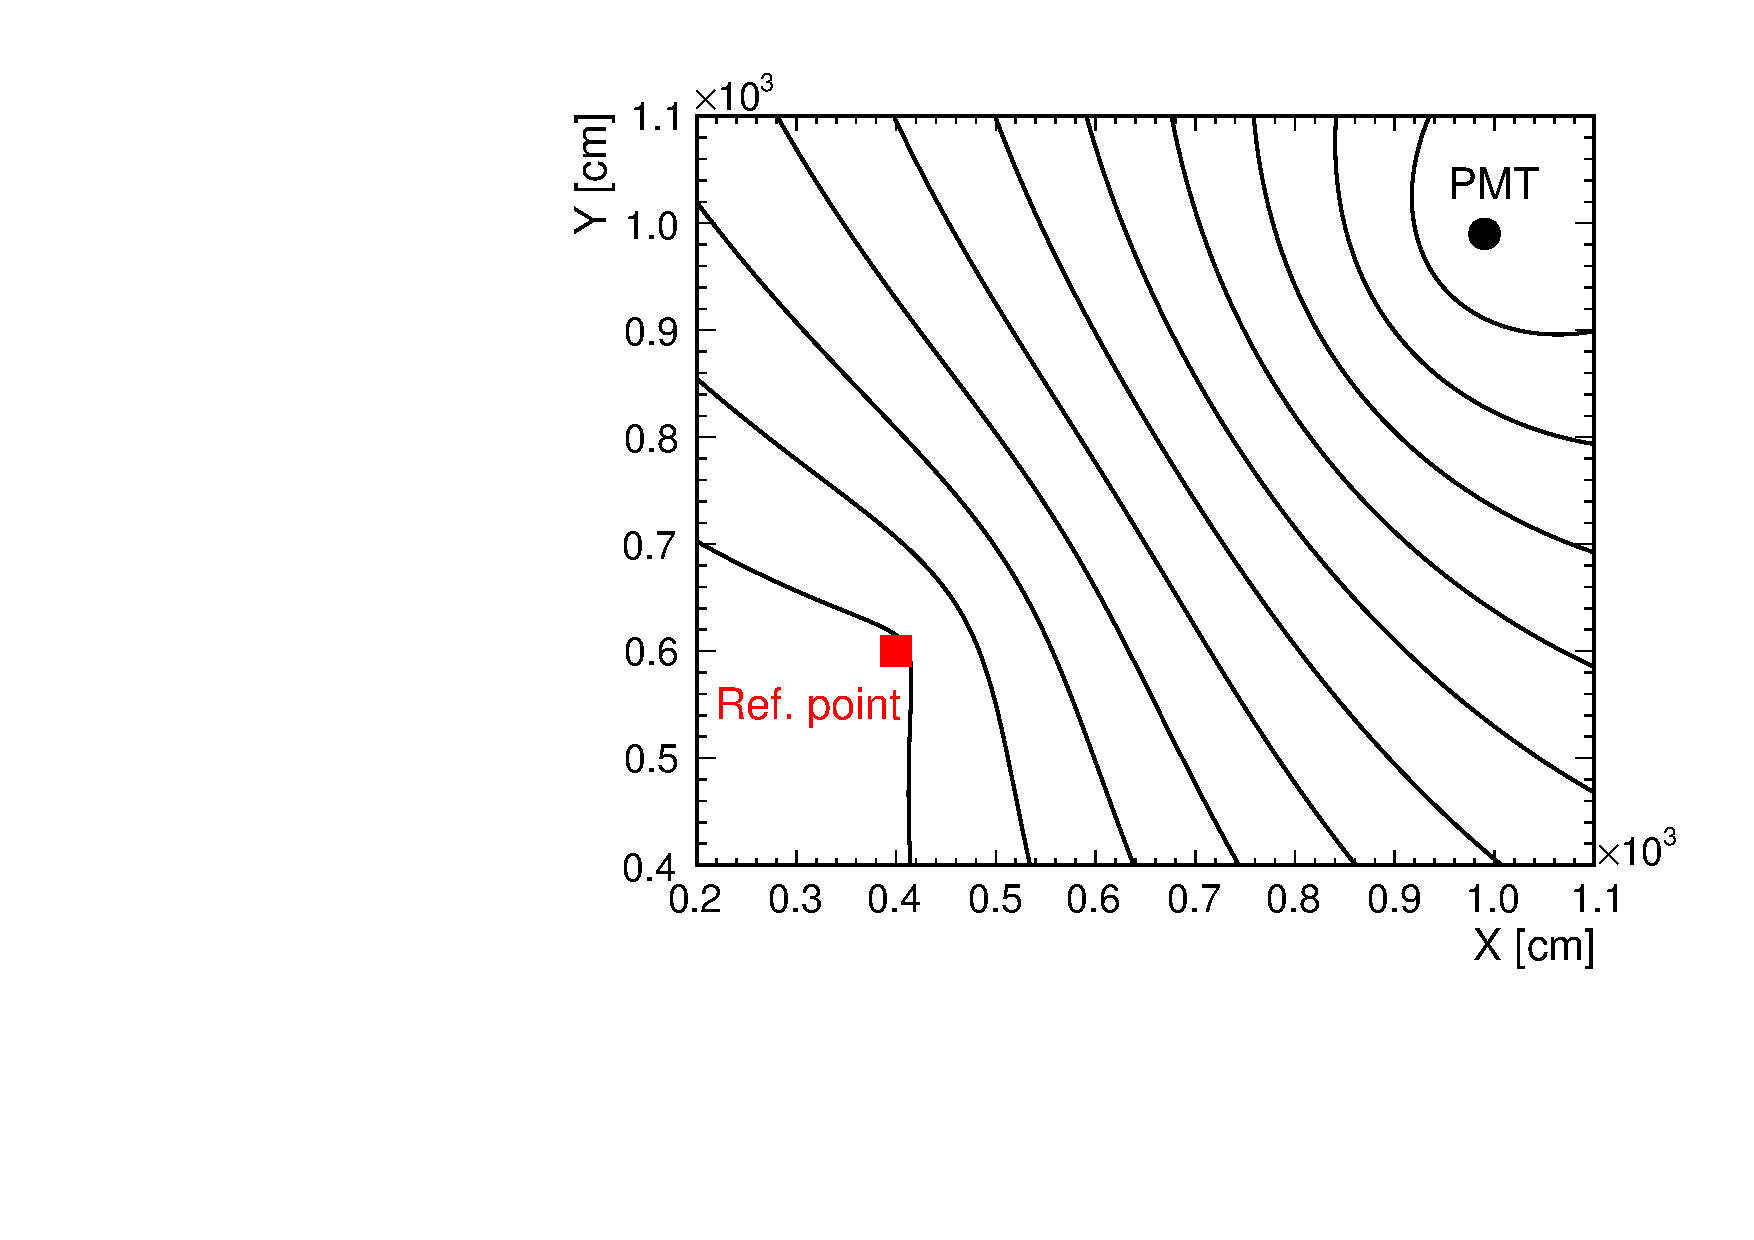
\includegraphics[trim=0.1cm 0.1cm 0.5cm 0.1cm,clip=true,width=\textwidth]
      {recon/DropShape_backward.pdf}
  \end{subfigure}
  \caption{
Isochrones in 2D for different values of $\hat{t}_j(\bvec{x})$ from 
\eqref{eq:RecoTimeModel} with the plus (left) or minus (right) sign for the term describing the 
particle contribution. In the computation of $\hat{t}_j(\bvec{x})$ relative to the reference point 
(red square) at $(400, 600)$\unit{cm}, $t_s$ was set to zero and 
$t_{\mathrm{ph}}(\bvec{x},\bvec{r}_j)$ was calculated as the time of flight for a direct path from 
$\bvec{x}$ to the photosensor (black circle) located at $(990, 990)$\unit{cm}. For simplicity, the 
phase velocity $v=c_0 / n$ with the refractive index $n = 1.484$ was used for the photon.}
  \label{fig:DropShapes}
\end{figure}
% ---------- FIGURE END ----------%
  
  The next important aspect that has to be considered is the quality of the time signal. In reality, the signal time will not correspond
  perfectly to the sum of particle and photon propagation time, but rather will follow a certain time distribution. Thus, in general 
  the emission point will not lie exactly on the drop-like surface. To take this into account, the drop-like shape has to be smeared 
  with the time distribution of the signals expected from the detector properties. In other words, the infinitesimally thin 
  surface aquires a profile. The shape of this profile perpendicular to the surface is given by the expected
  time distribution. A suitable time distribution for scintillation light is a convolution of a Gaussian, representing the time resolution of the photo 
  detectors, and an exponential function, representing the emission time of scintillation photons due to de-excitation with different 
  time constants:
  
  \begin{equation}
  \label{Eq:ScintillationTimeProfile}
 %  F(t) = \sum_{i} a_i \cdot \frac{\lambda_i}{2} \cdot e^{-\lambda_i (t - \frac{\lambda_i \sigma^2}{2})} \cdot \left[ 1 + erf(\frac{t - \lambda_i \sigma^2}{\sqrt{2} \sigma}) \right]
   F(t) = \sum_{i} a_i \cdot \frac{\lambda_i}{2} \cdot e^{-\lambda_i ((t - t_{signal}) - \frac{\lambda_i \sigma^2}{2})} \cdot \left[ 1 + erf(\frac{(t - t_{signal})- \lambda_i \sigma^2}{\sqrt{2} \sigma}) \right]
  \end{equation}
  %
  Here $\lambda_i = 1/\tau_i$ is the $i$-th decay constant of the scintillator and $a_i$ is the fraction of the corresponding decay 
  component with $\sum_{i} a_i = 1$. In total, we get a probability density distribution describing the probability 
  of a signal photon to be emitted from a given point $X$, which can be written as
  
  %The total score for each point $x$ in the detector 
  
  \begin{equation}
    \label{Eq:Raw_prob_density}
    P(\vec{x}) = F(t(\vec{x})) = F\left( (\abs{|\overline{VX}|} + n \cdot \abs{|\overline{XP}|})/c \right) \; .
  \end{equation}
  %
 % However, this formula is still incomplete since it can be more or less likely for a photon to come from certain parts of the drop-like shape depending on their
 % position with respect to the PMT.
  
  However, this formula is still incomplete since the probability of a photon to originate from certain parts of the drop-like shape
  also depends on their position with respect to the PMT. 
  %It is for example more likely that a photon will be detected that originates from a point directly in front of the PMT, where the effective PMT area is optimal,
  %than from an angle at the edge of the acceptance of the light concentrator. In other words, light distribution effects have to be included into the  
  %3d probability density distribution. 
  Effects to be considered are: The signal attenuation in the liquid scintillator, the effective PMT area depending on the distance and 
  the angle of a given point with respect to the PMT, and an angular acceptance function representing the optical properties of the PMT 
  and its light concentrator as well as any other aspect of the detector geometry such as shadowing. Also, the composition of the 
  detector has to be considered at this point: For example, in some experiments a buffer region generating much less light is present. 
  Concentrating these light distribution effects within the local detection efficiency $LD(\vec{x})$, we can rewrite Equation \ref{Eq:Raw_prob_density} as:
%  buffer region generating much less light is present, so that it is equaly less likely for a photon to originate from there. Concentrating these light distribution effects 
%  within the function $LD(\vec{x})$, we can rewrite equation \ref{Eq:Raw_prob_density} as:
  
  \begin{equation}
    \label{Eq:SinglePhotonDistribution_wo_PM}
    P(\vec{x}) = F(t(\vec{x})) \cdot LD(\vec{x}) \; .
  \end{equation}
  %
  At last this has to be normalised for each signal, leading to
  
  \begin{equation}
    \label{Eq:NormalisedSinglePhotonDistribution_wo_PM}
  %  P(\vec{x}) = \frac{F(t(\vec{x})) \cdot LD(\vec{x})}{\int_V F(t(\vec{x})) \cdot LD(\vec{x})  \cdot d\vec{x}} \; .
    P(\vec{x}) = \frac{F(t(\vec{x})) \cdot LD(\vec{x})}{\iiint F(t(\vec{x})) \cdot LD(\vec{x})  \cdot d\vec{x}} \; .
  \end{equation}
  %
  The resulting probability density distribution for a single signal is depicted in Fig. \ref{fig:SmearedDropShape} showing the effect of the time 
  distribution (left panel) and the additional influence of the light propagation effects (right panel).
  
  
  To finally get a 3D topological picture of the event, the 3D probability density distributions of all signals belonging to the event
  have to be combined. Since we do not know which photons have been emitted from the same point, all signals have to be considered as 
  being independent. Thus, the 3d probability density distributions of all signals have to be summed up:
  
  \begin{equation}
  %  \langle N_{photons} \rangle =  % nicht richtig, da man dazu ueber das Volumen integrieren muss
     P(\vec{x})_{total} = \sum_{i} P_i(\vec{x}) = \sum_{i} \left[ \frac{F_i(t(\vec{x})) \cdot LD_i(\vec{x})}{\iiint F_i(t(\vec{x})) \cdot LD_i(\vec{x})  \cdot d\vec{x}} \right] \; .
  \end{equation}
  %
%  Here, the index $i$ indicates the individual signal and the $F_i$ have to be evaluated with the position $P_i$ of the PMT which detected the signal and with $t_{signal, i}$, 
  Here, the index $i$ indicates the individual signals. Thus the $F_i$ have to be evaluated with the individual signal times $t_{signal, i}$ 
  and the position $P_i$ of the PMT which detected the signal, 
 % while $LD_i$ depends only on $P_i$. Therefore, it is convenient to group the signals by PMTs, so that equation \ref{} can be written as
%  while $LD_i$ depends only on $P_i$. %Therefore, it is convenient to group the signals by PMTs:
  while $LD_i$ is an attribute of this PMT depending on its position, optics and sensitivity. 
  
  % ---------- FIGURE BEGIN ----------%
\begin{figure}[b!t]
  \centering
  \begin{subfigure}[t]{0.48\textwidth}     
    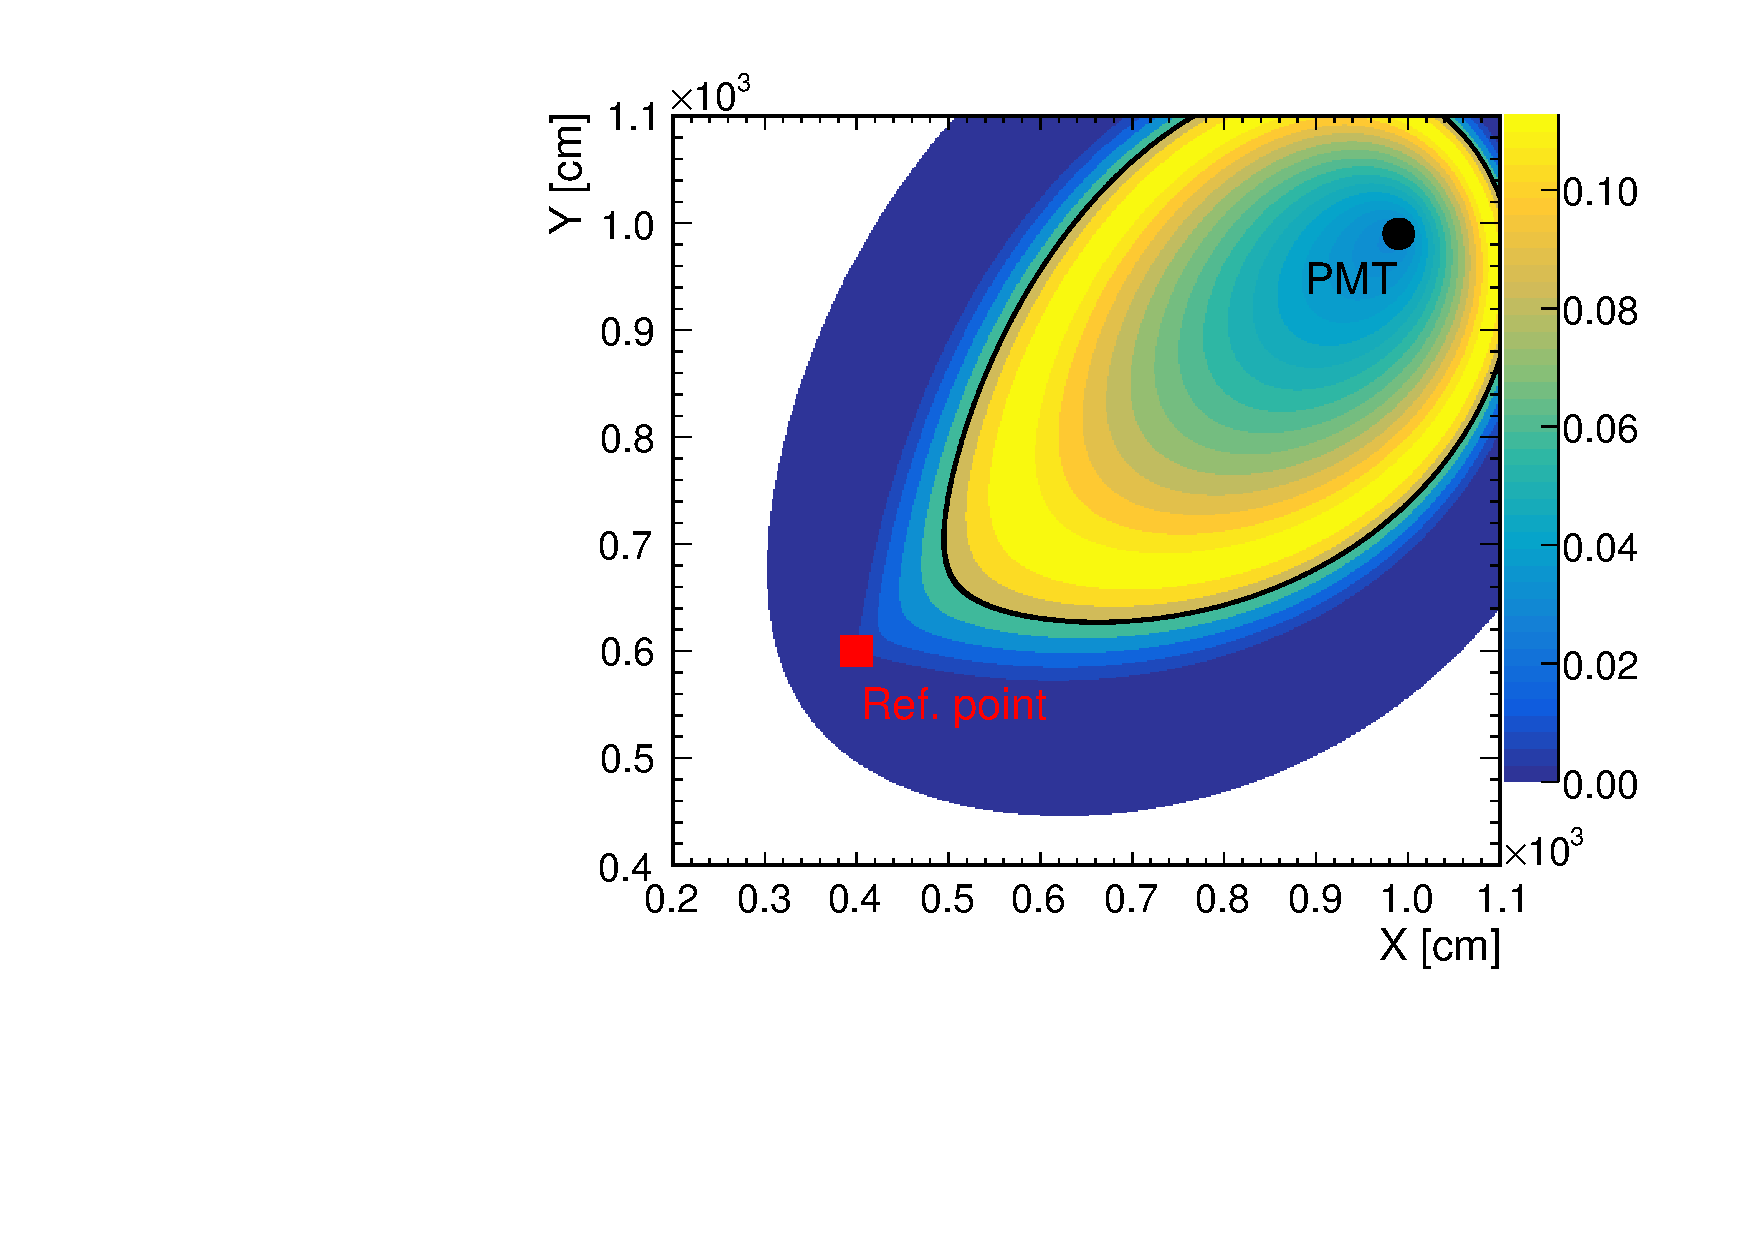
\includegraphics[trim=0.1cm 0.1cm 0.0cm 0.1cm,clip=true,width=\textwidth]
      {recon/SmearedDropShapeII.pdf}
  \end{subfigure}
  ~
  \begin{subfigure}[t]{0.48\textwidth}
    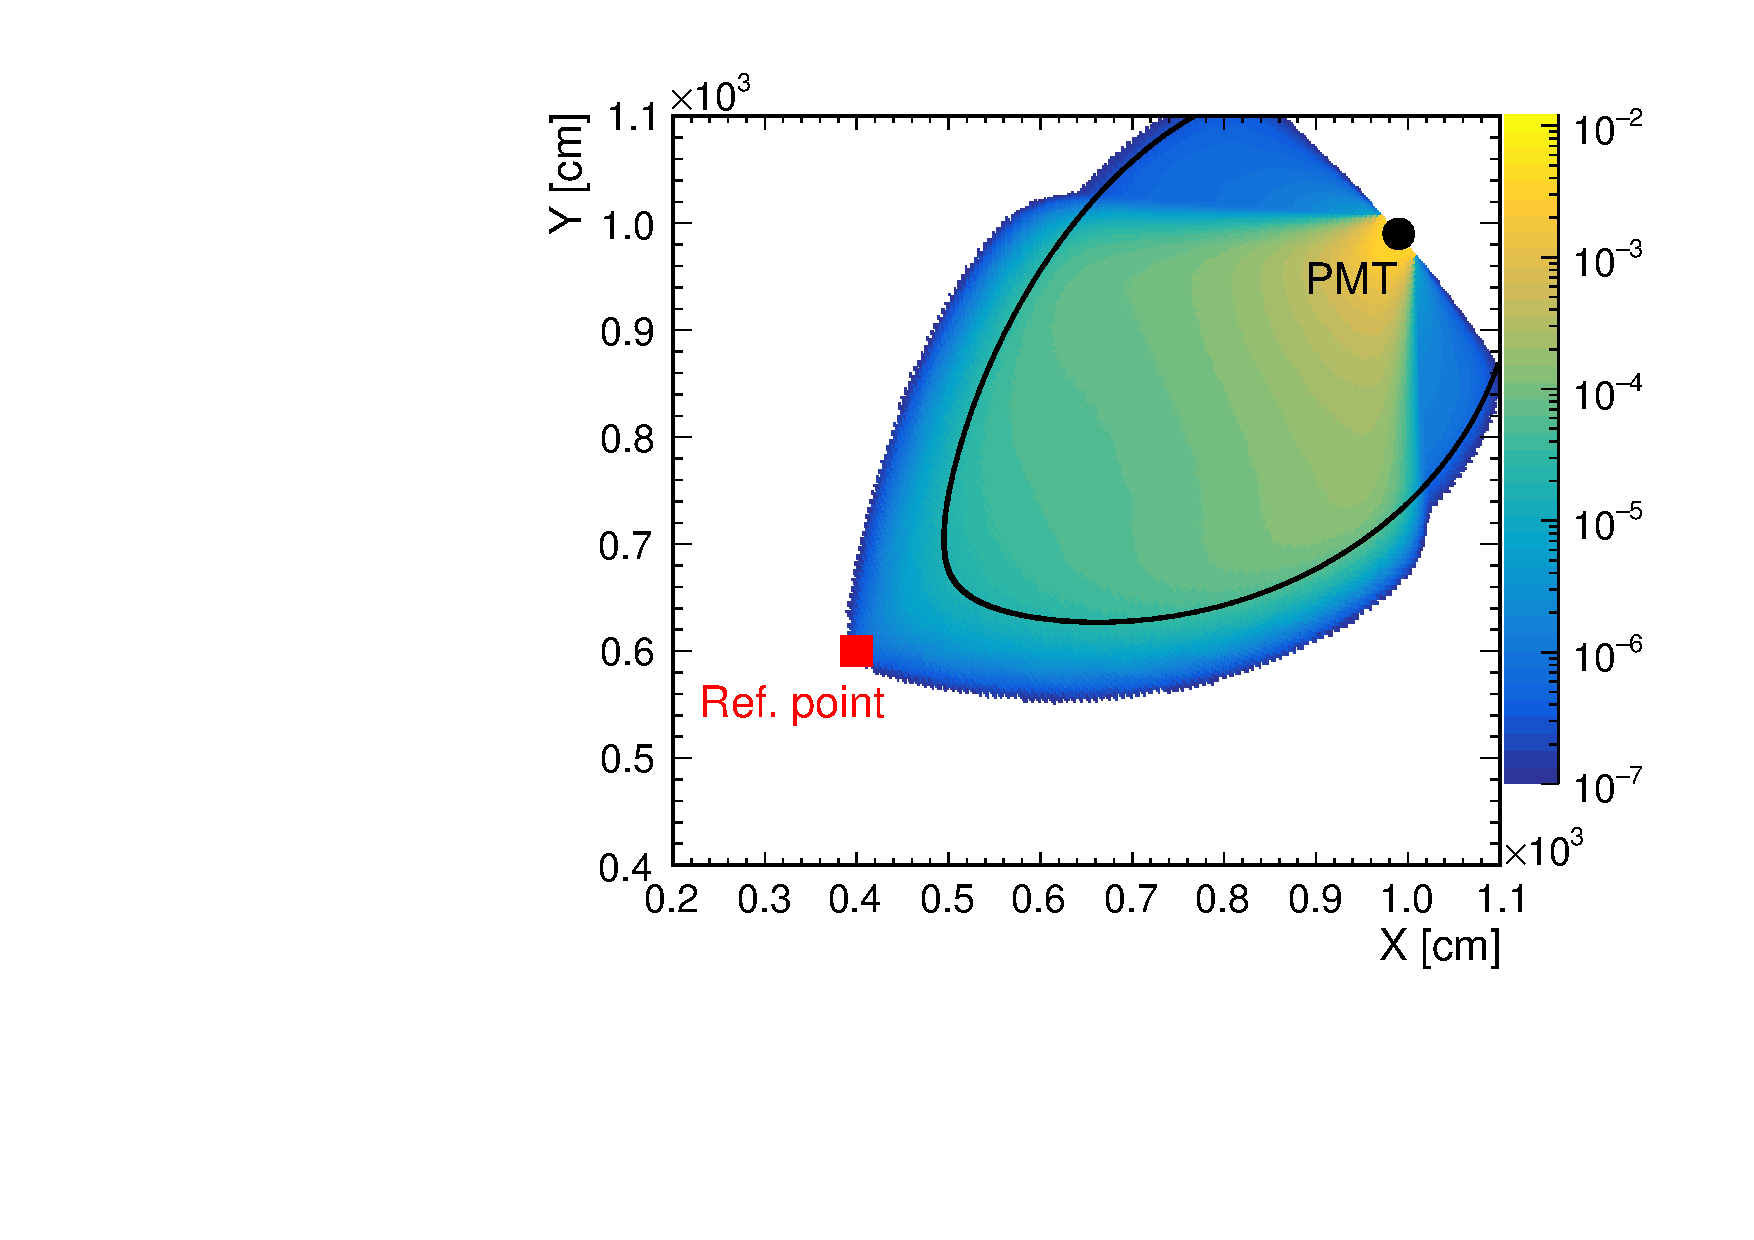
\includegraphics[trim=0.1cm 0.1cm 0.0cm 0.1cm,clip=true,width=\textwidth]
      {recon/SmearedDropShapeLDII.pdf}
  \end{subfigure}
  \caption{Unnormalized 2D versions of $\Phi_{j,k}(\bvec{x})$ with (right) and without (left) the 
inclusion of the spatial probability $P_{\mathrm{det},j}(\bvec{x})$ for the same configuration of 
photosensor and reference point as in \figref{fig:DropShapes}. The photon hit time for the sharp 
isochrone (black line), calculated as in \figref{fig:DropShapes} with the plus sign for the 
particle contribution, was set to $33$\unit{ns}.}
  \label{fig:SmearedDropShape}
\end{figure}
% ---------- FIGURE END ----------%
%  
%  \begin{equation}
%    P(\vec{x})_{Total} = \sum_{}  \; .
%  \end{equation}
%  
  The result is a 3d map of the expected mean number of detected photons $\langle N_{detected}(\vec{x}) \rangle$ coming from a given point. However, to get an impression of the energy
  deposition for a given event, not the number of detected photons from a given point is deciding but rather the number of photons emitted from that point $\langle N_{emitted}(\vec{x}) \rangle$.
  Therefore, every point of the 3d distribution has to be weighted by the inverse of the total signal detection efficiency $\eta(\vec{x})$ at that point:
  
  \begin{equation}
     \langle N_{emitted}(\vec{x}) \rangle = \frac{\langle N_{detected}(\vec{x}) \rangle}{\eta(\vec{x})} = \frac{P(\vec{x})_{total}}{\sum_{PMT} LD_{PMT}(\vec{x})}
  \end{equation}
  
  
  In principle, the reconstruction is completed at this point. However, due to the large width of the time distribution of the individual signals, the picture may not seem very
  sharp. On the other hand, the large number of photons involved still generates a very good spatial resolution of the event topology.
%  To extract this information further algorithm similiar to 2d image processing algorithms like filtering are neccessary, for example ridge-line finding, Sobel filter, etc. . 
  To extract this information, further algorithms are neccessary. For this purpose, standard algorithms developed originally for 2D image processing - like filtering, ridge-line finding,
  Sobel filter, etc. - can be adapted to accommodate 3D data.
  
  \subsection*{Iteration procedure}
  
  %To increase the quality of the picture
  
  So far, the individual 3D probability density distributions of all available signal photons have been added to get the total picture. 
  This is the correct way - from the statistics point of view - if all signals are completely independent of each other. In contrast, if
  all signals are directly correlated, as is the case for a point-like event, the individual 3D probability distributions can be multiplied
  in order to get the most likely common point of origin in the most efficient way. For extended events, this is not possible, because 
  not all of the signals belong to the same point. Then again, every point of the true event-topology is the origin of many detected photons
  and thus a correlation exist between these signals. In other words we have a mixure of correlated and uncorrelated information and need a 
  way to exploit the correlation.
  
  One way to take this into account is to divide the detector PMT-wise into equivalent subdetectors. If all of these subdetectors have enough signals to provide information about every point
  of the event topology, it is a robust approach to perform the above reconstruction for each of the subdetectors and then multiply the 3d topological distributions of all the 
  subdetectors. In this way, the topological information gets much sharper. However, this also introduces a bias, as points which are already more prominent in the
  individual results of the subdetectors will be artificially enhanced.
  
  To avoid this, another approach is followed here. The correlation we want to exploit is our knowledge that all signals belong to the same event and thus the same 
 % The correlation we want to exploit is our knowledge that all signals belong to the same event and thus the same 
  topology. If we dispose of a certain prior knowledge about that topology, we can express this as a 3D probability density distribution $PM(\vec{x})$. Instead of calculating 
  our topological 3D-picture from the completely independent 3D probability density distributions $P(\vec{x})_{i}$, we can now calculate this topology under the condition that it has to match 
  our knowledge $P(\vec{x}|PM(\vec{x}))_{i}$. In other words, if we already have a 3d representation of the event, which we call in this context probability mask ($PM$), we can use
  this to reweight the 3D probability density distribution generated by every single photon prior to its normalisation: Thus Equation 
  \ref{Eq:NormalisedSinglePhotonDistribution_wo_PM} becomes
  
  \begin{equation}
     P(\vec{x}|PM(\vec{x}))_{i} = \frac{F_{i}(t(\vec{x})) \cdot LD_{i}(\vec{x}) \cdot PM(\vec{x})}{\iiint F_{i}(t(\vec{x})) \cdot LD_{i}(\vec{x}) \cdot PM(\vec{x}) \cdot dV}
  \end{equation}
  
  In principle, the choice of the probability mask is free, as long as it represents the prior knowledge of the event in an unbiased way.
  For example the results of the likelihood method in Section \ref{} could be used to predefine a volume where to look for energy 
  depositions. The easiest way to generate a $PM$ is then to give every point inside the volume of interest the value 1 and set the 
  probability outside to zero. However, it turns out that sharp edges may negatively affect the reconstruction result: In this case,
  the normalisation enhances signals too much which only have a slight overlap with the $PM$. This often happens with signals from 
  scattered photons, as they do not carry any topological information on the event and thus are only noise for the reconstruction. One
  way to cure this is to smoothen the edges of the selected region by adding a region where the PM slowly goes to zero, for instance a 
  Gaussian flank. 
  %Of course the output of the other to algorithms can directly be used as a $PM$, but as they use only the first hit of each PMT, their output has to be modified to avoid a bias occuring from this.
  
  A natural choice is to use the reconstruction as described in Section \ref{Sec:BasicWonsakReco}, i.e. without a $PM$, first. The result
  of this reconstruction then constitutes an unbiased representation of the event topology, which can then be used as the $PM$ for a second
  iteration of the reconstruction. The result of this second reconstruction can again be fed back as a new $PM$ into the reconstruction 
  process. Thus an iterative procedure is created. The power of this iterative process can be seen in Fig. \ref{fig:RecoItrResults}. Ultimately, this allows
  a close association of each signal photon with a certain volume of the event topology. This makes the energy deposition per unit length 
  accessible as can bee seen in Fig. \ref{fig:RecoItrResults}. 
  
  To improve the robustness and the convergence speed of the iteration procedure, we applied an additional artifice to produce the results 
  presented in \ref{fig:RecoItrResults}: If the full reconstruction result is used for the $PM$ of the next iteration a small impreciseness enters the 
  procedure. The reason for this is that the data used, was also used to generate the $PM$ and the two are thus not completely independent
  from each other. This can lead to self-enhancement effects, if a certain region of the 3d probability density distribution under 
  inspection is dominated by data from a single source (PMT). To avoid this, in principle every PMT would need its own $PM$, generated with
  the help of all the other PMTs. This however is impractical. A more convenient solution is to divide the dataset into two completely 
  independent parts being as similar as possible, e.g. by just taking every second PMT for each part respectively. Then one of these 
  datasets can be used to produce the $PM$ for the other half of the PMTs and the other way round. By alternating between the
  two datasets in the iterative procedure self-enhancement can be suppressed. To use the full dataset for the final result, the last two
  iteration outputs must then be combined by adding them up.
  % ---------- FIGURE BEGIN ----------%
\begin{figure}[b!t]
  \centering
  \begin{subfigure}[t]{0.99\textwidth}     
    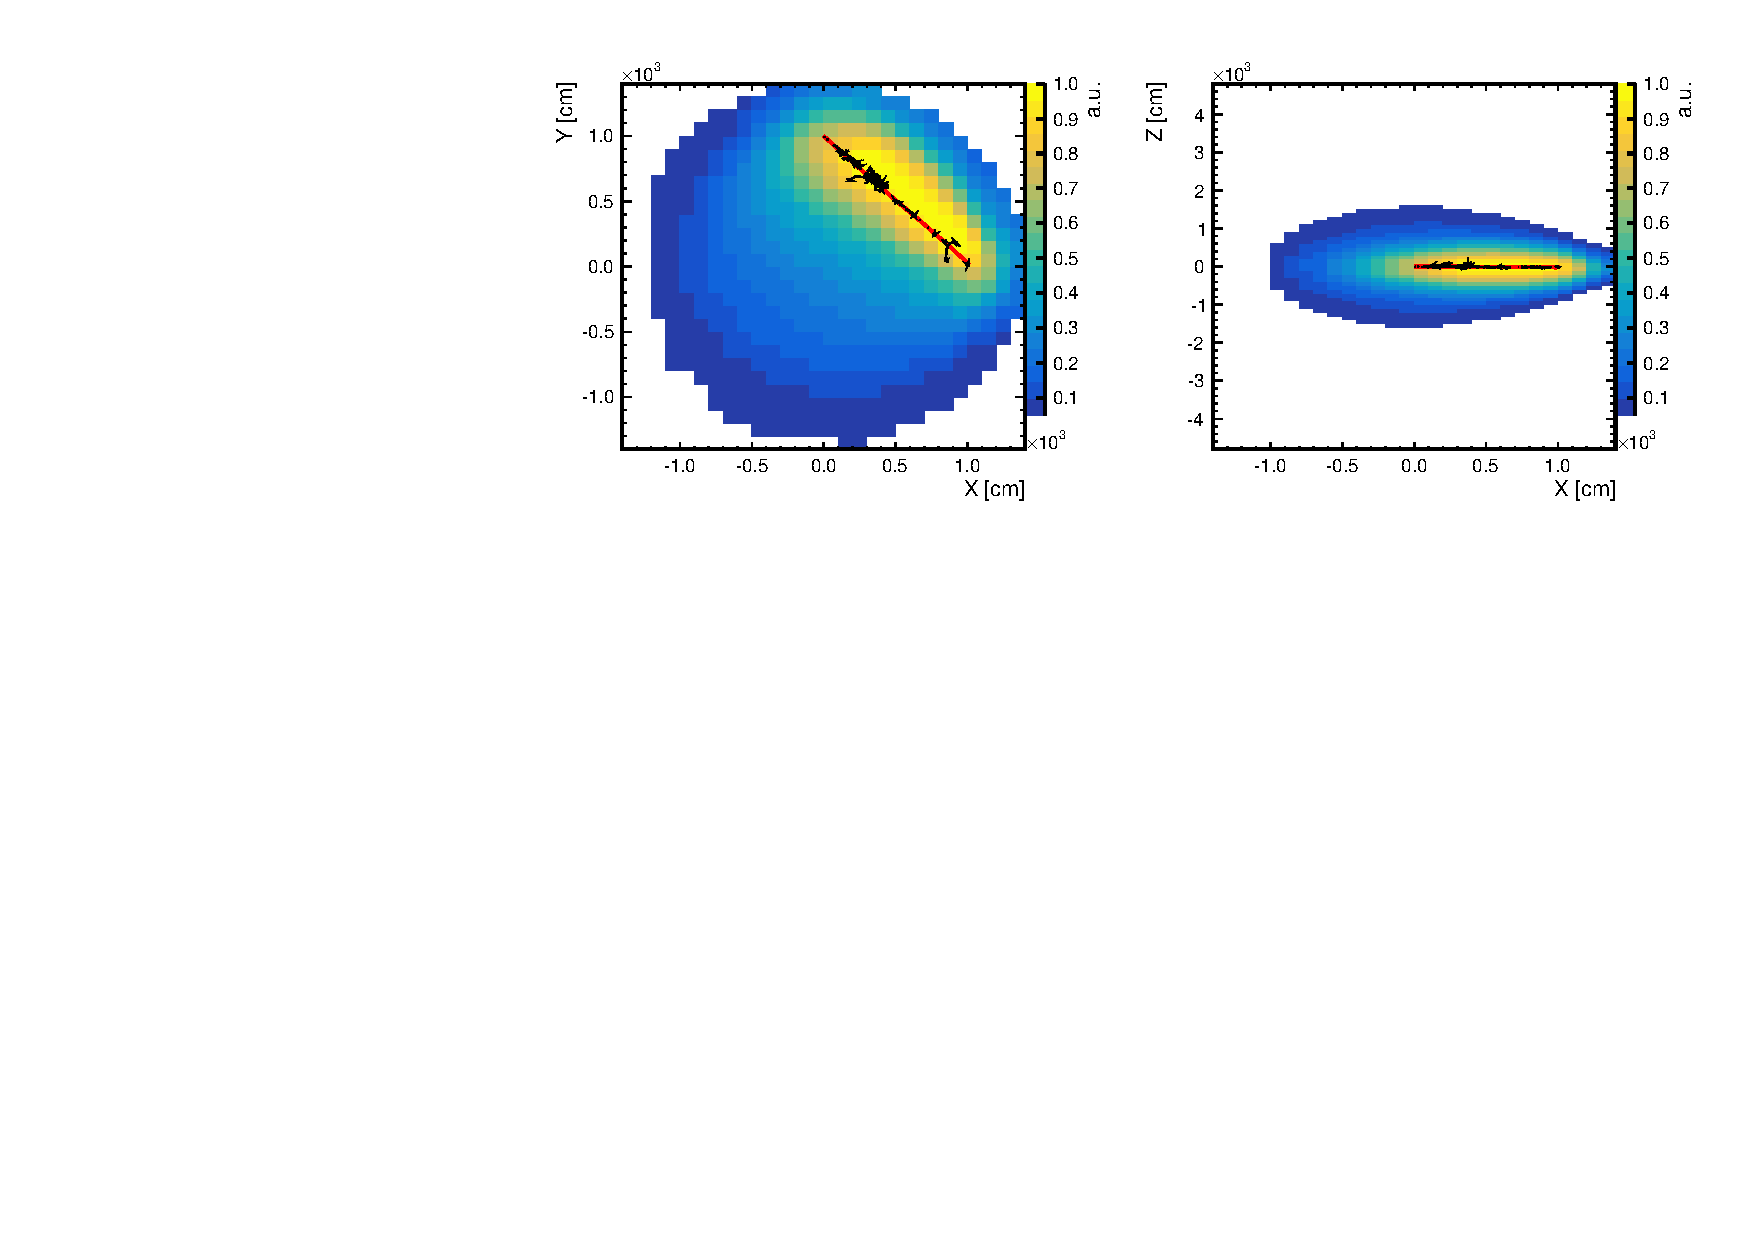
\includegraphics[trim=0.1cm 0.1cm 0.0cm 0.1cm,clip=true,width=\textwidth]
      {recon/RecoResult0.pdf}
  \end{subfigure}
  ~
    \begin{subfigure}[t]{0.99\textwidth}     
    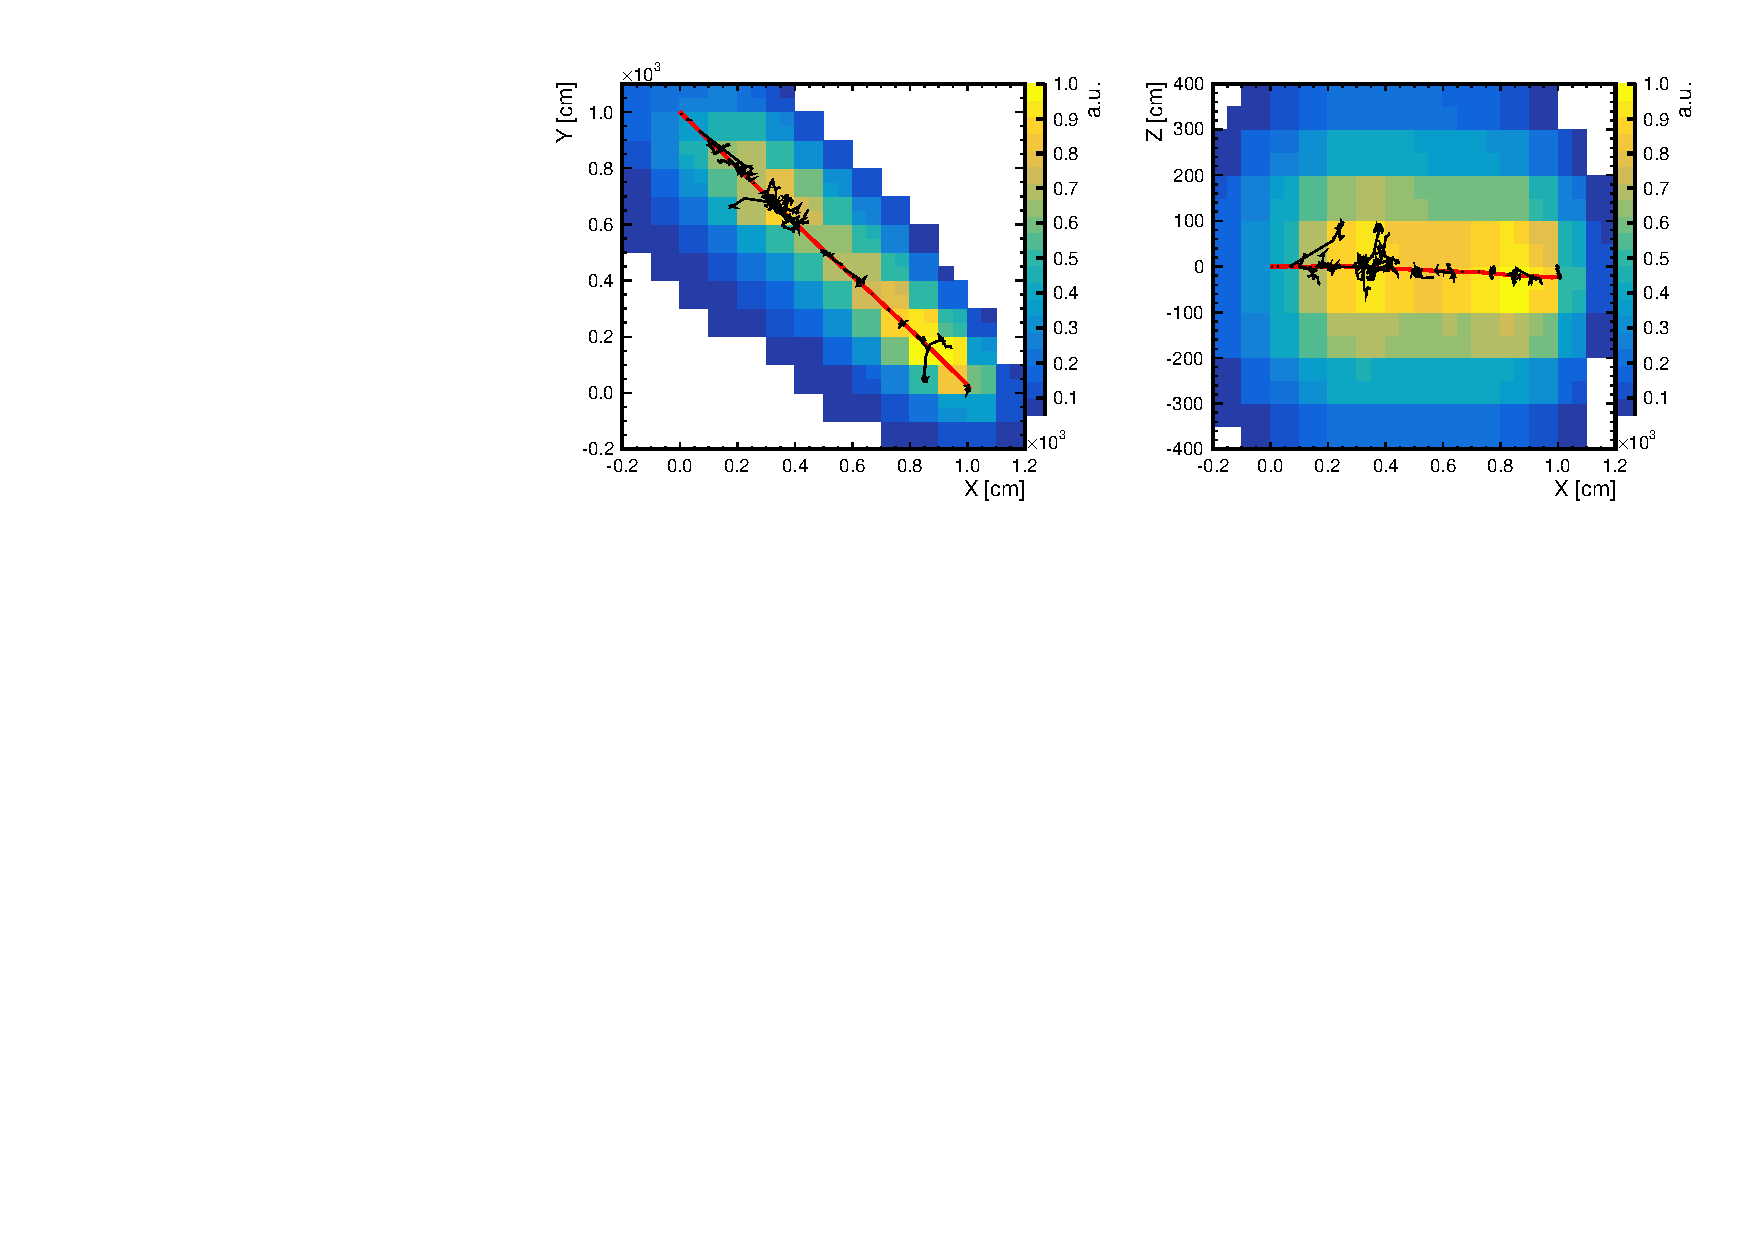
\includegraphics[trim=0.1cm 0.1cm 0.0cm 0.1cm,clip=true,width=\textwidth]
      {recon/RecoResult8.pdf}
  \end{subfigure}
  ~
  \begin{subfigure}[t]{0.99\textwidth}
    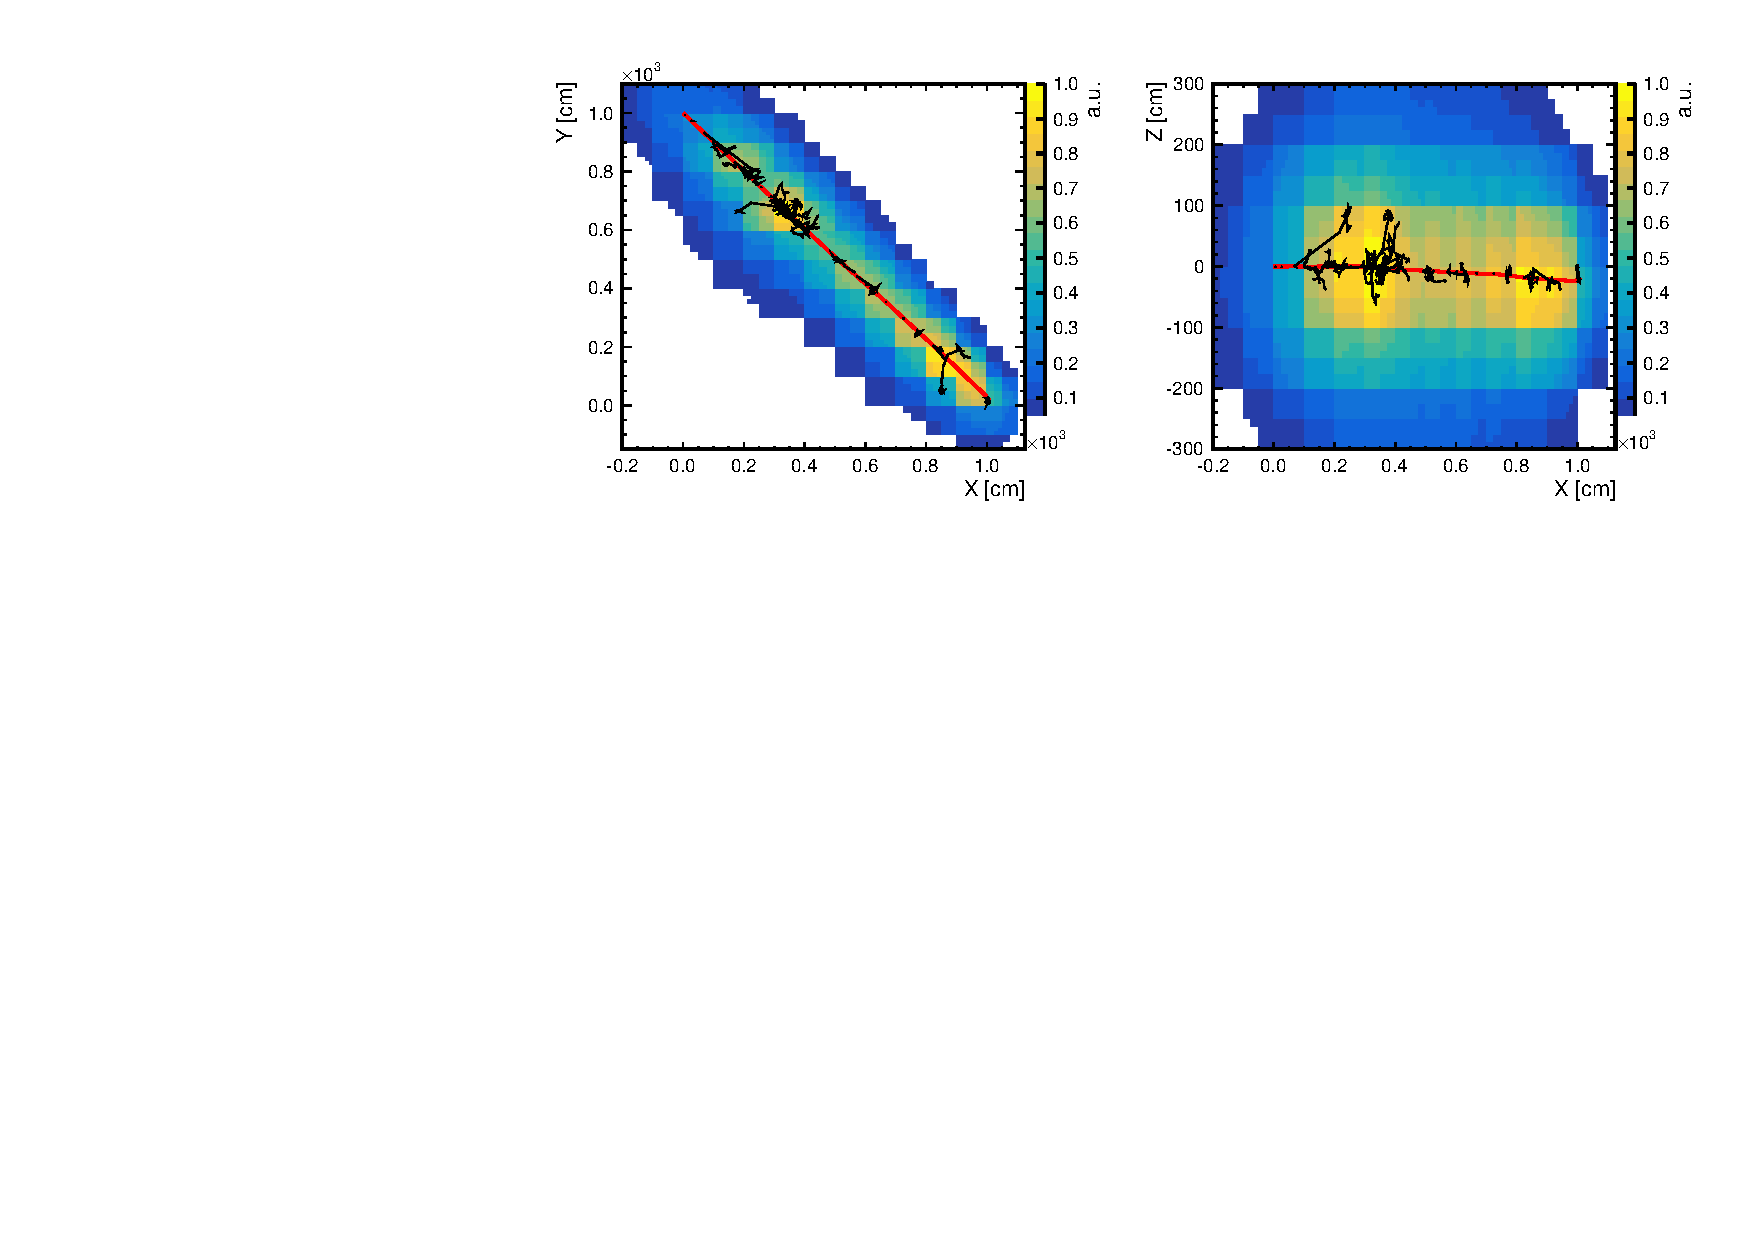
\includegraphics[trim=0.1cm 0.1cm 0.0cm 0.1cm,clip=true,width=\textwidth]
      {recon/RecoResult21.pdf}
  \end{subfigure}
  \caption{Reconstruction results after the iterations 0 (top), 8 (middle) and 21 (bottom) for a 
simulated muon with $3$\unit{GeV} initial kinetic energy in the cylindrical LENA detector projected 
along the symmetry axis (left) or a radial $y$-axis (right). The primary particle started at 
$(0,\,1000,\,0)$\unit{cm} in the direction $(1,\, -1,\, 0)$. Both the projected tracks of the 
primary particle (red) and of secondary particles (black) are shown. Note that both the axis scales 
and the sizes of the cells change due to the selection of a region of interest and the refinement 
of the reconstruction mesh. Moreover, the cell content is given in a.u. and rescaled such that the 
maximum content is $1$. Some details on the actual reconstruction procedure are given in
\secref{sec:Reconstruction}.
}
  \label{fig:RecoItrResults}
\end{figure}
% ---------- FIGURE END ----------%
  %Trick mit der zweiteilung
  
  %But, as these algorithms use only the first hit of 
 % each PMT the representation of the event they give is not unbiased concerning the context here. Still they can be used to define volume of interest
  
 % multiplication of subsamples?
  
  
  
  
  
  
 % backward in time
 % any reference point
 % reference point from backtracking or other sources

  
 %  In combination with the fact that the photons are not 
 % produced instantaneusly, but with decay constants of the order of a few ns, this leads to large uncertainties of the time information. 
  
%  scattering?
  
  \subsection*{Short summary}
  
  The whole procedure can be put into this logical sequence:
  
  \begin{enumerate}
   \item Get a reference point
   \item Calculate drop-like surface for each signal
   \item Smear the surface with the time profile of the signals
   \item Add light distribution effects
   \item Normalise the probability density distribution for each signal 
   \item Use the spatial-dependent light detection efficiency to go from detected light to emitted light
   \item Use the result of emitted light as a probability mask and repeat everything starting from point 5
 %  \item cleaning  
 %  \item crystalisation
  \end{enumerate}

  Since the probability mask will only start to affect everything during the normalisation of the single photon probability density distributions,
  the iteration can in principle begin at point 5 of this sequence. However, this is very memory intensive, since the raw results of each PMT have
  to be saved (the 3d representation of equation \ref{Eq:SinglePhotonDistribution_wo_PM}). Thus we choose to begin the iteration loop at point 2. 
  
  %However, due to memory limitations of the computer involved it has so far been necessary in our case to begin the iteration process at point 2. \textcolor{red}{last sentence might not be true, still hav eto think about it}
  
 % \begin{itemize}
 % \end{itemize}
 
 
 %technical realisation
  
  \subsection*{Results}
  
  So far this method has mainly been studied with the help of the LENA simulation. This simulation includes only an effective optical model and 
  no Cherenkov light. Furthermore, it was assumed that every photon could be registered separatly. LENA has a coverage of ~30\% resulting in 
  approximatly 250 detected photons per MeV. To reduce the computation time for the reconstruction an adaptive mesh was used. This allowed to 
  establish a voxel size of 12.5 cm in the final iteration. More details about the simulation and the technical implementation of the topological
  reconstruction can be found in \ref{}.
  
  To proof the robustness and show the potential of this method a large sample of fully contained muons with energies between 1 and 10 GeV was 
  used. An angular resolution between 1.4° at 1~GeV and 0.4° at 10~GeV could be achieved. 
  
 %Verweis auf unser paper -> apadtive mesh, unhit PMTs
  
 % MC used
 % Muon Energy and Angular resolution
 % Electron and Muon Separation
 % Picture Theia event
  
  %\subsection{Application to MeV events}
  
  \subsection*{Application to Cherenov-light}
  
  Some modifications are needed for the application of this method to Cherenkov light. The most obvious one is the 
  time profile $F(t)$ (equation \ref{Eq:ScintillationTimeProfile}), since the Cherenkov process emits 
  the light instantaneously. Thus in most scenarios the timing profile of the photosensors will be the dominant
  factor, which can often be described by a Gaussian with the corresponding time resolution. However, chromatic 
  dispersion of the Cherenkov light must be taken into account if sensors with very good time resolution 
  (below 1 ns) are employed in detectors of the size of THEIA. 
  
  In addition the position dependent detection efficiencies also become direction dependent now, since the Cherenkov 
  light is emitted only in a cone with respect to the particle direction. How to generate such direction dependent
  detection efficiencies is shown for example in \cite{}. However, in general they differ for different particles
  due to the different behaviour when passing through matter. Thus smaller or wider angular distributions of the emitted
  Cherenkov light are generated. This is the same effect that allows to distinguish between electrons and muons 
  based on the sharpness of the Cherenkov ring.
  
  Since the idea of this method is to work without any hyphothesis, such a situation is unfortunate. To avoid
  this, we start instead with the basic method without any light distribution effect (detection efficiencies). Thanks to 
  the good timing quality of the Cherenkov-light this already allows to define an accurate region of interest. Now, we 
  calculate the angular distribution (with respect to the direction to the reference point) of all the signals for every
  point (voxel) in this region of interest. However, for each point we use only signals that match the point in time 
  (the isochrone  of the signal time representing equation \ref{Eq:Drop-like_shape} is close enough to the point). This 
  angular distribution can then be used to calculate the local detection efficiency for each PMT at this position in the 
  detector. Once we have this we can proceed with the same iteration process used for the scintillation light.
  
  %-> Probability to be Cherenkov!
  
 % This is then working well if the method without the iteration process is used. To get reliable results with the whole procedure it is
  
  \subsection*{Separation of Cherenkov and scintillation light}
  

 
 % Ablaufdiagram
  
%\subsection{Adding light distribution effects}

%\subsection{Normalisation}

%\subsection{Probability Mask}

%\subsection{Edge finding}

%\subsection{Results for muons}

%\subsection{Potential}


%\subsection{Backtracking}

\subsection{Low energies reconstruction} 

by Andrey

%
%\newpage
%
%% \input{conclusion/outlook.tex}
%
%% BIBLIOGRAPHY
%%__________________________________________________________________________________________________%
%\addcontentsline{toc}{section}{Bibliography}
%\bibliographystyle{unsrt}
%\bibliography{bib/bibliographyV2}
%
%
%% DOCUMENT END
%%==================================================================================================%
%\end{document}
%%==================================================================================================%